% ------------------------------------------------------------------------------
% ------------------------------------------------------------------------------
% Relatório do Exercício 3 de Algoritmos Numéricos 2
% Autor: André Barreto Silveira
% ------------------------------------------------------------------------------
% ------------------------------------------------------------------------------

\documentclass[
	11pt,				% tamanho da fonte
	oneside,			% para impressão apenas no verso. Oposto a twoside
	a4paper,			% tamanho do papel. 
	english,			% idioma adicional para hifenização
	brazil,				% o último idioma é o principal do documento
	]{article}


% ---
% PACOTES
% ---
\usepackage{lmodern}
\usepackage[T1]{fontenc}
\usepackage[utf8]{inputenc}
\usepackage{indentfirst}
\usepackage{nomencl}
\usepackage{color}
\usepackage{graphicx}
\usepackage{microtype}
\usepackage{makeidx}
\usepackage{multirow,tabularx}
\usepackage{multicol}
\usepackage{listings}
\usepackage{color}
\usepackage{hyperref}
\usepackage{cite}
\usepackage{url}
\usepackage[brazilian]{babel}
\usepackage[brazilian,hyperpageref]{backref}
\usepackage[fleqn]{amsmath}
\usepackage{mathtools,amssymb}
\usepackage{pgfplots}

\usepackage{lipsum}
% ---

% ---
% Configurações do pacote listings
% ---
\definecolor{mygreen}{rgb}{0,0.6,0}
\definecolor{mygray}{rgb}{0.571428571,0.571428571,0.571428571}
\definecolor{mymauve}{rgb}{0.5714285718,0,0.82}
\definecolor{codegreen}{rgb}{0,0.6,0}
\definecolor{codegray}{rgb}{0.571428571,0.571428571,0.571428571}
\definecolor{codepurple}{rgb}{0.5714285718,0,0.82}
\definecolor{backcolour}{rgb}{0.95,0.95,0.92}
\lstset{
	backgroundcolor=\color{white},
	basicstyle=\footnotesize,
	breakatwhitespace=false,
	breaklines=true,
	captionpos=b,
	commentstyle=\color{mygreen},
	deletekeywords={...},
	escapeinside={\%*}{*)},
	extendedchars=true,
	keepspaces=true,
	keywordstyle=\color{blue},
	language=C,
	otherkeywords={*,...},
	numbers=left,
	numbersep=5pt,
	numberstyle=\tiny\color{mygray},
	rulecolor=\color{black},
	showspaces=false,
	showstringspaces=false,
	showtabs=false,
	stepnumber=1,
	stringstyle=\color{mymauve},
	tabsize=2,
	title=\lstname
}
% ---
	
% ---
% Informações de dados para CAPA
% ---
\title{\textbf{Solução de Problemas de Valor no Contorno Bidimensionais}}
\author{
André Barreto e Igor Ventorim\\\\
\normalsize Universidade Federal do Espírito Santo\\
}
\date{2015}
% ---

% ---
% Configurações de aparência do PDF final
% ---
\definecolor{blue}{RGB}{41,5,195}

% informações do PDF
\makeatletter
\hypersetup{
	pdftitle={\@title}, 
	pdfauthor={\@author},
	pdfsubject={Escalonamento de Jobs},
	pdfcreator={LaTeX with abnTeX2},
	pdfkeywords={abnt}{latex}{abntex}{abntex2}{atigo científico}, 
	colorlinks=true,
	linkcolor=blue,
	citecolor=blue,
	filecolor=magenta,
	urlcolor=blue,
	bookmarksdepth=4
}
\makeatother
% --- 

% ---
% Compila o indice
% ---
\makeindex
% ---

% --- 
% Espaçamentos entre linhas e parágrafos 
% --- 
\setlength{\parindent}{1cm}
\setlength{\parskip}{0.2cm}
% ---

% ----
% Início do documento
% ----
\begin{document}
% ---

% Seleciona o idioma do documento
\selectlanguage{brazil}

% Retira espaço extra obsoleto entre as frases.
\frenchspacing

\graphicspath{ {Imagens/} }

% ------------------------------------------------------------------------------
% Página de Título
% ------------------------------------------------------------------------------
\begin{titlepage}
	\centering
	{\scshape \large Universidade Federal do Espírito Santo\par}
	{\large Departamento de Informática\par}
	\vspace{1cm}
	{\large André Barreto Silveira\par}
	
	\vfill
	
	{\LARGE \bfseries Equação do Calor Unidimensional Transiente\par}
	\vspace{1cm}
	{\large Exercício 3 de Algoritmos Numéricos 2\par}

	\vfill

	{\large Vitória\par}
	{\large 2016\par}
\end{titlepage}
\addtocounter{page}{1}

% ------------------------------------------------------------------------------
% Introdução
% ------------------------------------------------------------------------------
\section{Introdução}
Neste documento serão apresentados os testes numéricos dos algoritmos 
explícito, implícito e de Crank-Nicolson para resolver a equação de calor 
unidimensional pelo método das diferenças finitas.

% ------------------------------------------------------------------------------
% Teste Numéricos
% ------------------------------------------------------------------------------
\section{Testes Numéricos}

\subsection{Teste 1}

Equação do calor com condutividade térmica $a(x,t) = 0.835 cm^2/s$ e fonte de 
calor nula:

\begin{itemize}
 \item Parâmetros básicos:
 $a(x,t) = 0.835$, $f(x,t) = 0$, $(0,l) = (0,10)$ e número de passos no tempo 
igual a 60.
 \item Condições de contorno e iniciais:
 $u(0,t) = 100ºC$, $u(10,t) = 50ºC$ e $u(x,0) = 0$, para $x \in (0,10)$
 \item Parâmetros dos métodos de aproximação:
 \begin{itemize}
  \item $h = 1$ e $\Delta t_1 < \frac{h^2}{2a}$, $\Delta t_2 = 
\frac{h^2}{2a}$, $\Delta t_3 > \frac{h^2}{2a}$
  \item $h = 0.1$ e $\Delta t_1 < \frac{h^2}{2a}$, $\Delta t_2 = 
\frac{h^2}{2a}$, $\Delta t_3 > \frac{h^2}{2a}$
 \end{itemize}
\end{itemize}	

\begin{figure}[h]
    \centering
    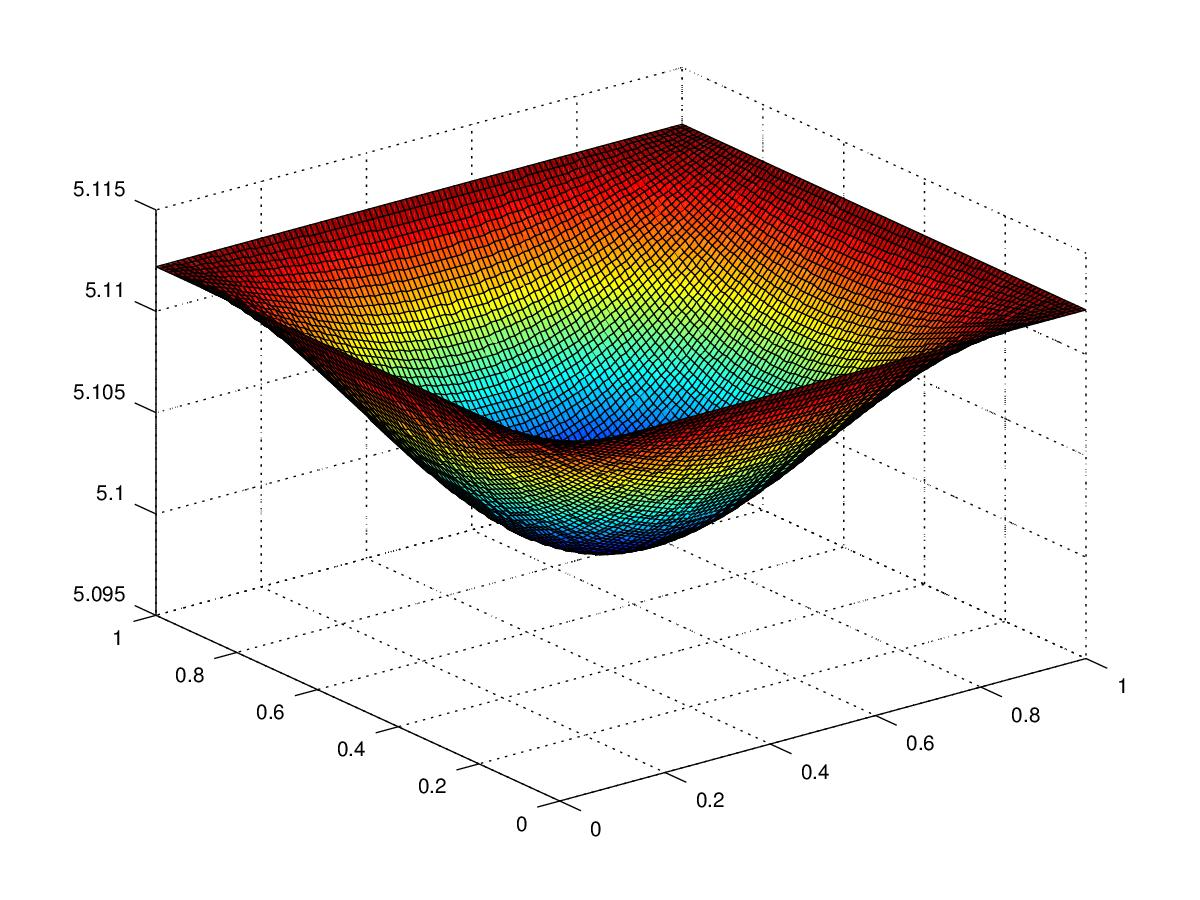
\includegraphics[width=0.8\textwidth]{v1_100-100.jpg}
    \caption{Gráfico solução da Validação 1 para $n = 100$ e $m = 100$}
    \label{fig:v1_100-100}
\end{figure}

\subsection{Teste 2}
Neste experimento, deve-se determinar a solução aproximada para $u(x,y)$ em 
$\Omega = (0,1) \times (0,1)$ considerando na Eq.

\begin{figure}[h]
    \centering
    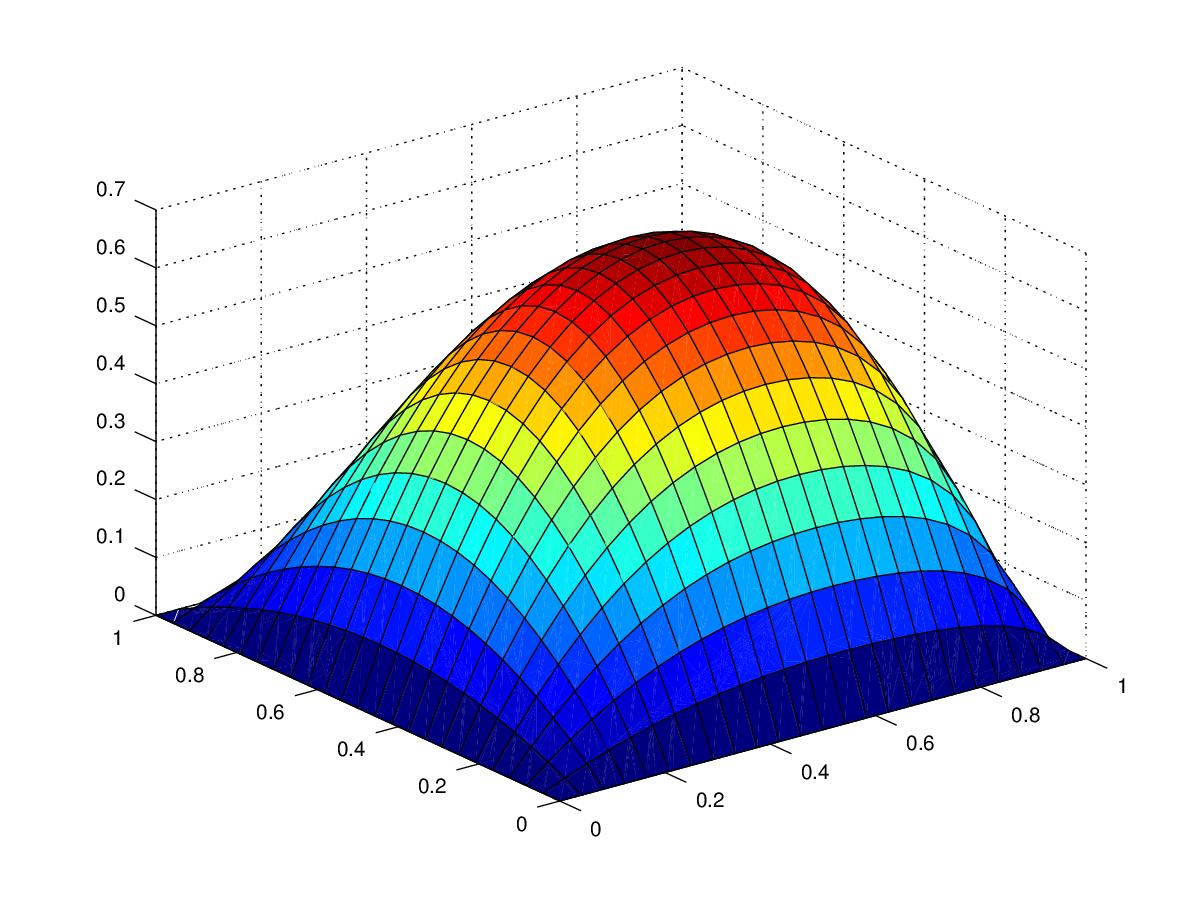
\includegraphics[width=0.8\textwidth]{v2_25-25}
    \caption{Gráfico solução da Validação 2 para $n = 25$ e $m = 25$}
    \label{fig:v2_25-25}
\end{figure}

\begin{figure}[h]
    \centering
    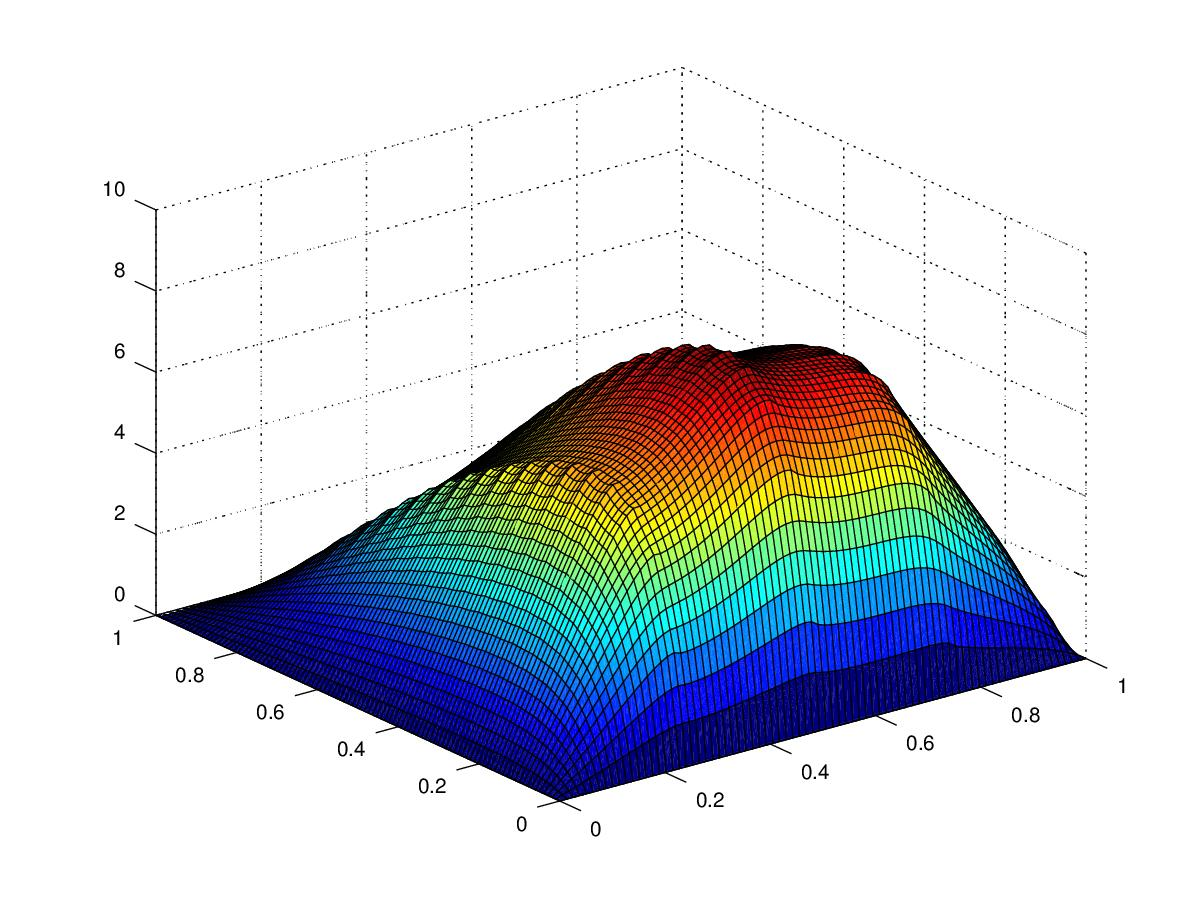
\includegraphics[width=0.8\textwidth]{v2_80-100}
    \caption{Gráfico solução da Validação 2 para $n = 80$ e $m = 100$}
    \label{fig:v2_80-100}
\end{figure}

\subsection{Teste 3}
Este experimento consiste em uma aplicação dos métodos em questão para resfriar 
uma massa aquecida. Exemplos podem incluir o resfriamento de chips de 
computadores ou amplificadores elétricos. O modelo matemático que descreve a 
transferência de calor nas direções $x$ e $y$ é dado por:

Veja na figura \ref{fig:a1_25-25} o gráfico da solução encontrada ao aplicar 
a Aplicação Física 1 para $\Omega = (0,1)\times(0,1)$, $n = 25$ e $m = 25$, e 
na figura \ref{fig:a1_25-100} o gráfico da solução encontrada ao aplicar 
a Aplicação Física 1 para $\Omega = (0,1)\times(0,1)$, $n = 25$ e $m = 100$.

\begin{figure}[h]
    \centering
    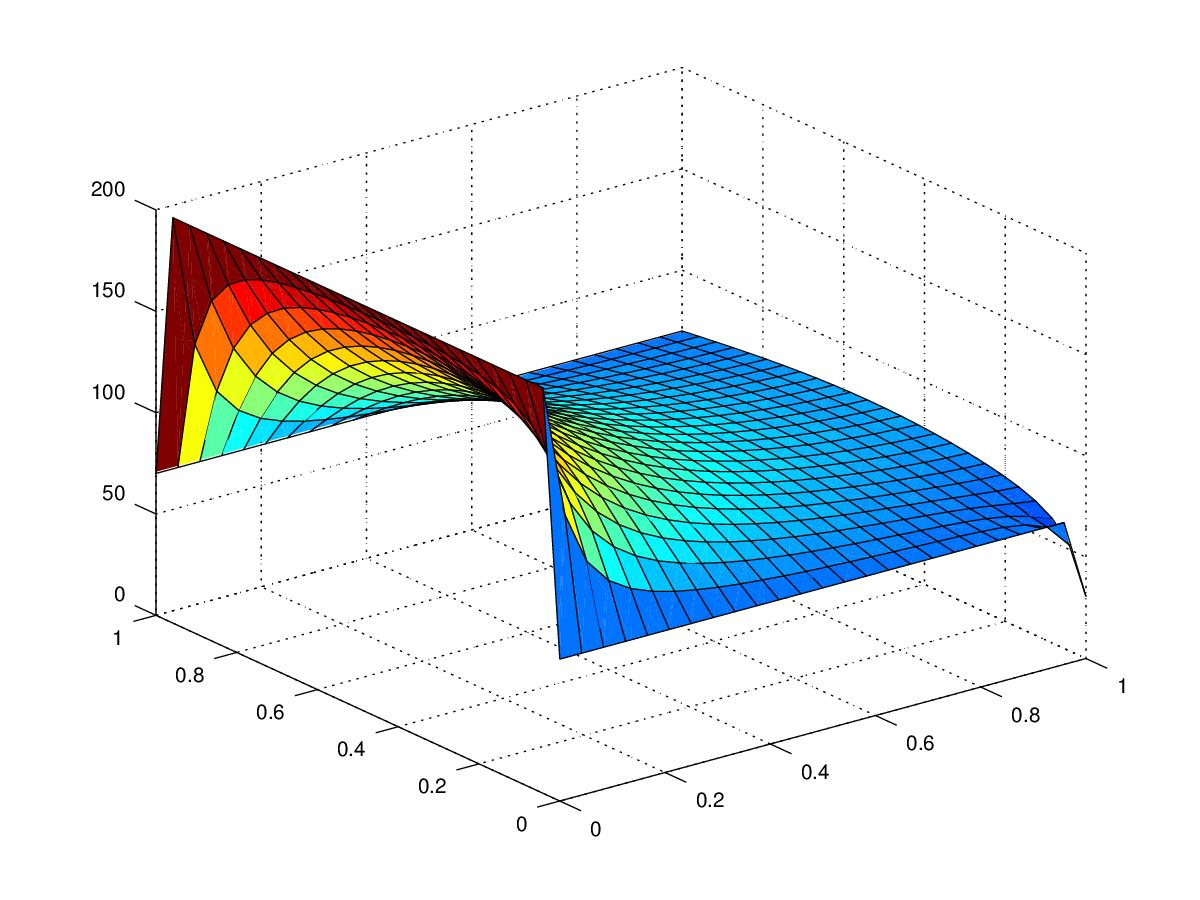
\includegraphics[width=0.8\textwidth]{a1_25-25}
    \caption{Gráfico solução da Aplicação Física 1 para $n = 25$ e $m = 25$}
    \label{fig:a1_25-25}
\end{figure}

\begin{figure}[h]
    \centering
    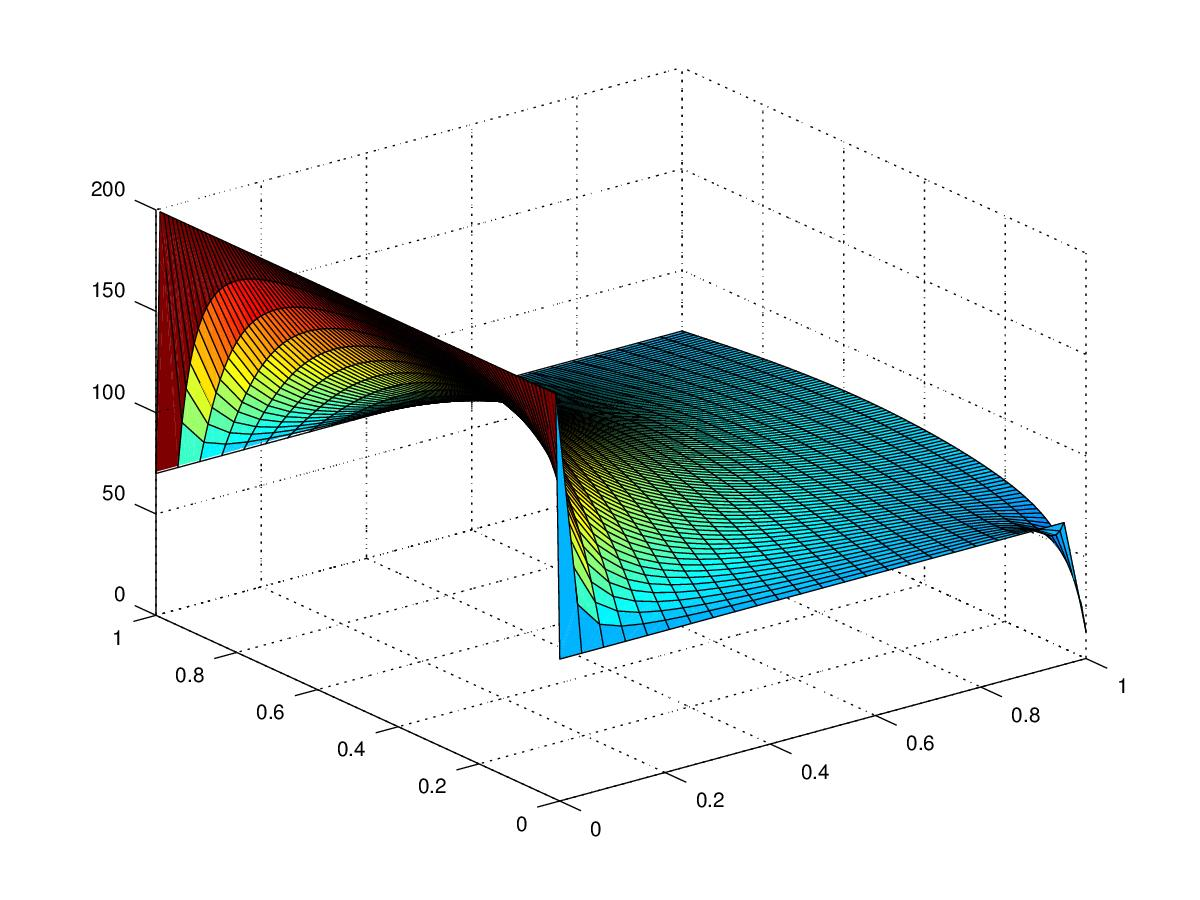
\includegraphics[width=0.8\textwidth]{a1_25-100}
    \caption{Gráfico solução da Aplicação Física 1 para $n = 25$ e $m = 100$}
    \label{fig:a1_25-100}
\end{figure}

Em ambos os testes anteriores, foi-se aplicado a condição de contorno mista. 
Caso seja aplicado a condição de contorno de valor prescrito $u(L, y) =
70$, e utilizando os dados $\Omega = (0,1)\times(0,1)$, $n = 25$ e $m = 100$, 
teremos um gráfico de solução ilustrado pela figura \ref{fig:a170_25-100}

\begin{figure}[h]
    \centering
    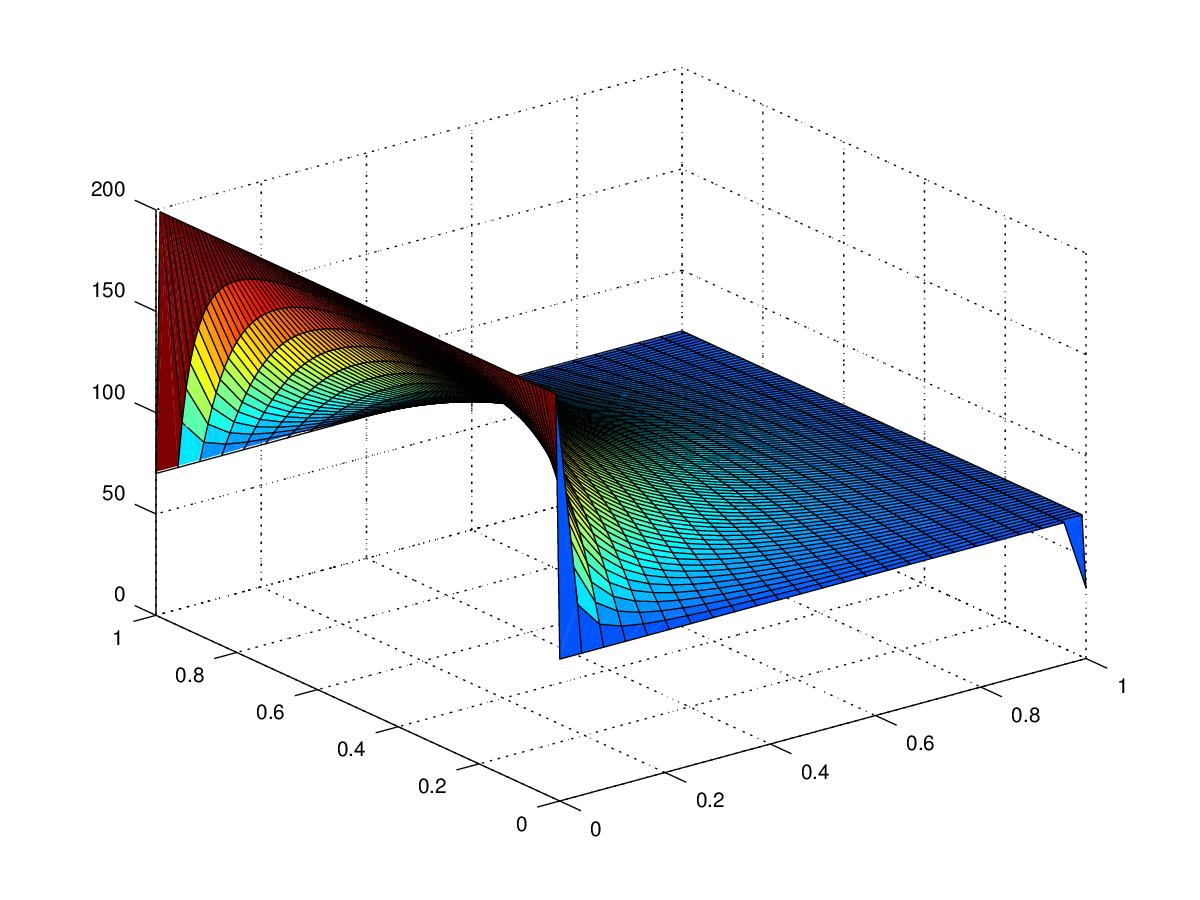
\includegraphics[width=0.8\textwidth]{a170_25-100}
    \caption{Gráfico solução da Aplicação Física 1 para $n = 25$ e $m = 100$ e 
$u(L, y) = 70$}
    \label{fig:a170_25-100}
\end{figure}

Podemos ver que as soluções encontradas para $n = 25$ e $m = 100$ modificando a 
condição de contorno são muito similares. Inclusive, a norma da solução é igual 
à 200.00 em ambos os casos. Um fato importante é notar que o caso de valor 
prescrito convergiu mais rapidamente (808 contra 1040 iterações do SOR).

% ------------------------------------------------------------------------------
% Conclusão
% ------------------------------------------------------------------------------
\section{Conclusão}
\lipsum[2]

\end{document}
